\documentclass{beamer}

\usepackage{amssymb,amsmath}
\usepackage{graphicx}
\usepackage{url}
\usepackage{color}
\usepackage{relsize}		% For \smaller
\usepackage{url}			% For \url
\usepackage{epstopdf}	% Included EPS files automatically converted to PDF to include with pdflatex

%For MindMaps
% \usepackage{tikz}%
% \usetikzlibrary{mindmap,trees,arrows}%

%%% Color Definitions %%%%%%%%%%%%%%%%%%%%%%%%%%%%%%%%%%%%%%%%%%%%%%%%%%%%%%%%%
%\definecolor{bordercol}{RGB}{40,40,40}
%\definecolor{headercol1}{RGB}{186,215,230}
%\definecolor{headercol2}{RGB}{80,80,80}
%\definecolor{headerfontcol}{RGB}{0,0,0}
%\definecolor{boxcolor}{RGB}{186,215,230}

%%% Save space in lists. Use this after the opening of the list %%%%%%%%%%%%%%%%
%\newcommand{\compresslist}{
%	\setlength{\itemsep}{1pt}
%	\setlength{\parskip}{0pt}
%	\setlength{\parsep}{0pt}
%}

%\setbeameroption{show notes on top}

% You should run 'pdflatex' TWICE, because of TOC issues.

% Rename this file.  A common temptation for first-time slide makers
% is to name it something like ``my_talk.tex'' or
% ``john_doe_talk.tex'' or even ``discrete_math_seminar_talk.tex''.
% You really won't like any of these titles the second time you give a
% talk.  Try naming your tex file something more descriptive, like
% ``riemann_hypothesis_short_proof_talk.tex''.  Even better (in case
% you recycle 99% of a talk, but still want to change a little, and
% retain copies of each), how about
% ``riemann_hypothesis_short_proof_MIT-Colloquium.2000-01-01.tex''?

\mode<presentation>
{
  % A tip: pick a theme you like first, and THEN modify the color theme, and then add math content.
  % Warsaw is the theme selected by default in Beamer's installation sample files.

  %%%%%%%%%%%%%%%%%%%%%%%%%%%% THEME
  %\usetheme{AnnArbor}
  %\usetheme{Antibes}
  %\usetheme{Bergen}
  %\usetheme{Berkeley}		% bem bacana - menu esquerdo
  %\usetheme{Berlin}
  %\usetheme{Boadilla}
  %\usetheme{boxes}
  %\usetheme{CambridgeUS}		% bem bacana - menu superior
  %\usetheme{Copenhagen}
  %\usetheme{Darmstadt}
  %\usetheme{default}
  %\usetheme{Dresden}
  \usetheme{Frankfurt}
  %\usetheme{Goettingen}
  %\usetheme{Hannover}		% bem bacana - menu esquerdo
  %\usetheme{Ilmenau}
  %\usetheme{JuanLesPins}
  %\usetheme{Luebeck}
  %\usetheme{Madrid}		%bacana
  %\usetheme{Malmoe}
  %\usetheme{Marburg}		% bem bacana - menu direito
  %\usetheme{Montpellier}
  %\usetheme{PaloAlto}		% bem bacana - menu esquerdo
  %\usetheme{Pittsburgh}
  %\usetheme{Rochester}		%bacana
  %\usetheme{Singapore}
  %\usetheme{Szeged}
  %\usetheme{Warsaw}

  %%%%%%%%%%%%%%%%%%%%%%%%%%%% COLOR THEME
  %\usecolortheme{albatross}		% azul escuro, massa
  %\usecolortheme{beetle}		% cinza, menu azul
  %\usecolortheme{crane}		% branco e amarelo, massa
  \usecolortheme{default}		% branco, azul clarinho
  %\usecolortheme{dolphin}		% azul e branco, legal
  %\usecolortheme{dove}			% cinza e branco, feio
  %\usecolortheme{fly}			% todo cinza, horrível
  %\usecolortheme{lily}			% parece o default
  %\usecolortheme{orchid}		% azul e branco, ok
  %\usecolortheme{rose}			% branco e violeta-claro, bonito
  %\usecolortheme{seagull}		% cinza, feio
  %\usecolortheme{seahorse}		% nhé, meio feio
  %\usecolortheme{sidebartab}		% Azul, branco, destaque na tab, interessante
  %\usecolortheme{structure}		% bichado
  %\usecolortheme{whale}		% Azul e branco, bem bonito

  %%%%%%%%%%%%%%%%%%%%%%%%%%%% OUTER THEME
  \useoutertheme{default}
  %\useoutertheme{infolines}
  %\useoutertheme{miniframes}
  %\useoutertheme{shadow}
  %\useoutertheme{sidebar}
  %\useoutertheme{smoothbars}
  %\useoutertheme{smoothtree}
  %\useoutertheme{split}
  %\useoutertheme{tree}

  %%%%%%%%%%%%%%%%%%%%%%%%%%%% INNER THEME
  \useinnertheme{circles}
  %\useinnertheme{default}
  %\useinnertheme{inmargin}
  %\useinnertheme{rectangles}
  %\useinnertheme{rounded}

  %%%%%%%%%%%%%%%%%%%%%%%%%%%%%%%%%%%

  \setbeamercovered{invisible} % or whatever (possibly just delete it)
  % To change behavior of \uncover from graying out to totally
  % invisible, can change \setbeamercovered to invisible instead of
  % transparent. apparently there are also 'dynamic' modes that make
  % the amount of graying depend on how long it'll take until the
  % thing is uncovered.

}


% Get rid of nav bar
\beamertemplatenavigationsymbolsempty

% Use short top
%\usepackage[headheight=12pt,footheight=12pt]{beamerthemeboxes}
%\addheadboxtemplate{\color{black}}{
%\hskip0.5cm
%\color{white}
%\insertshortauthor \ \ \ \ 
%\insertframenumber \ \ \ \ \ \ \ 
%\insertsection \ \ \ \ \ \ \ \ \ \ \ \ \ \ \ \ \  \insertsubsection
%\hskip0.5cm}
%\addheadboxtemplate{\color{black}}{
%\color{white}
%\ \ \ \ 
%\insertsection
%}
%\addheadboxtemplate{\color{black}}{
%\color{white}
%\ \ \ \ 
%\insertsubsection
%}

% Insert frame number at bottom of the page.
% \usefoottemplate{\hfil\tiny{\color{black!90}\insertframenumber}} 

\usepackage[english]{babel}
\usepackage[latin1]{inputenc}
\usepackage{subfigure}

\usepackage{times}
\usepackage[T1]{fontenc}


\title[GB21802]{GB21802 - Programming Challenges}
\subtitle[]{Week 1 - Data Structures}
\author[Claus Aranha]{Claus Aranha\\{\footnotesize caranha@cs.tsukuba.ac.jp}}
\institute{College of Information Science}
\date{2015-04-22,25\\{\tiny Last updated \today}}

\begin{document}

\section{Introduction}
\subsection{Title}
\begin{frame}
\maketitle
\end{frame}

\subsection{Notes and Warnings}

\begin{frame}
  \frametitle{Summary for Week 0}
  \begin{itemize}
  \item How the course works;
  \item How to solve simple (ad-hoc) programming challenges;
  \item Four simple programming challenges;
  \end{itemize}
\end{frame}

\begin{frame}
  \frametitle{Results for Week 0}
  \begin{tabular}{l|l|l|l|}
    Problem & Total& Submissions & Solutions\\
    \hline
    Division of Nlogonia & 31 & 27 & 27\\
    Cancer or Scorpio & 31 & 25 & 19 \\
    3n+1 Problem & 31 & 23 & 21 \\
    Request for Proposal & 31 & 18 & 13\\
    \hline
  \end{tabular}

  \bigskip
  \begin{center}
    Congratulations to all who submitted!

    \smallskip

    The problems for this week are already online.
  \end{center}
\end{frame}


\begin{frame}
  \frametitle{Outline for Week 1}

  \begin{block}{Week Theme: Data Structures}
  This week, we will review and discuss the different data structures that
  are often used in competitive programming problems.
  \end{block}

  \vfill

  \begin{itemize}
  \item Types and Variations of Data Structures (Linear 2D, 3D, Dynamic, Non-linear)
  \item Discussion on Implementation and notes;
  \item Discussion about next week exercises;
  \item Bitmasks (Monday?)
  \end{itemize}
\end{frame}


% Motivation to learn data structures
%% 8-queens example last week
%% Towers of hanoi example
%% Another example (Maybe File Fragmentation? -- maybe do this next week?)
\subsection{motivation}

\begin{frame}
  \frametitle{Motivation: Why study data structures?}

  \begin{itemize}
  \item The correct data structure makes the algorithm \structure{faster;}
    \smallskip
    {\small \emph{Example:} As we saw last week, the solution space of the 
      8-queen problem depends on the chosen structure.}

    \vspace{2em}

  \item A good \structure{implementation} of a data structure
    makes the implementation easier;

    \smallskip
    {\small \emph{Exemple:} Using a linked list, you raise the possibility of 
      null pointer errors.}
  \end{itemize}

  \begin{center}
    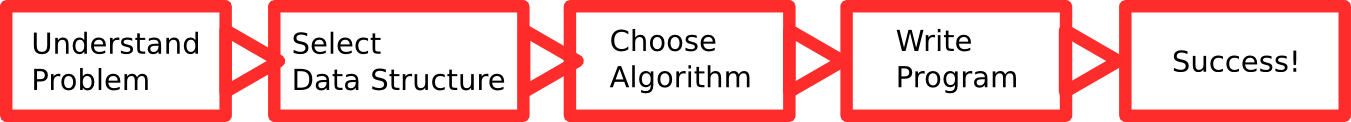
\includegraphics[width=0.8\textwidth]{../img/pipeline}
  \end{center}
  
\end{frame}

%% 8-queens example last week
%% Towers of hanoi example

\begin{frame}
  \frametitle{Example 1: 8 Queen Problem (UVA 750)}
  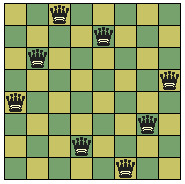
\includegraphics[width=.25\textwidth]{../img/8queen}\\
  Given the initial position of one queen, how many correct solutions exist?
  
  \begin{itemize}
  \item X,Y position representation = $58^8$ total solutions
  \item Column position representation = $8^8$ total solutions
  \item Permutation representation = $8!$ total solutions
  \end{itemize}


  \hrulefill\\
  {\tiny\hfill Image by Lee Daniel Crocker. CC-BY-SA 3.0}
\end{frame}

\begin{frame}
  \frametitle{Example 2: The Towers of Hanoi}
  
  \begin{center}
    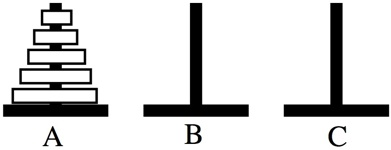
\includegraphics[width=0.5\textwidth]{img/hanoi}
  \end{center}
  \medskip

  {\small
    \begin{itemize}
    \item You have $N$ disks and $K$ poles. Each disk has unique size $s_i$.
    \item A disk $i$ can be moved from one pole to another.
    \item A move of disk $i$ to pole $k$ is only valid if $k$ has no disks smaller than $i$
    \item Find the list of moves to move all disks from pole 1 to pole $K$.
    \end{itemize}
  }
  
  \vfill

  How do you represent the data in this problem?
\end{frame}

\begin{frame}
  \frametitle{Another way to visualize the Towers of Hanoi}
  \begin{center}
    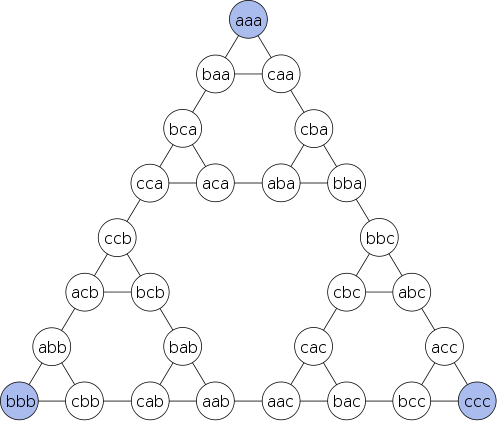
\includegraphics[width=0.7\textwidth]{img/hanoi_graph}
  \end{center}
  {\tiny \hfill Image created by nonenmac}
\end{frame}

\begin{frame}
  \frametitle{Explaining the Tower of Hanoi Data Structure}
  \begin{columns}[c]
    \column{0.7\textwidth}
    \begin{itemize}
    \item Each node identifies an state in the problem;
    \item Each character in the string represents one disk and its
      position;
    \item We can have at most 3 state transitions at each state (can
      you prove it?)
    \item To solve the Towers of Hanoi problem, we find the path
      between the start and end states.
    \item (just beware of state explosion)
    \end{itemize}
    \column{0.3\textwidth}    
    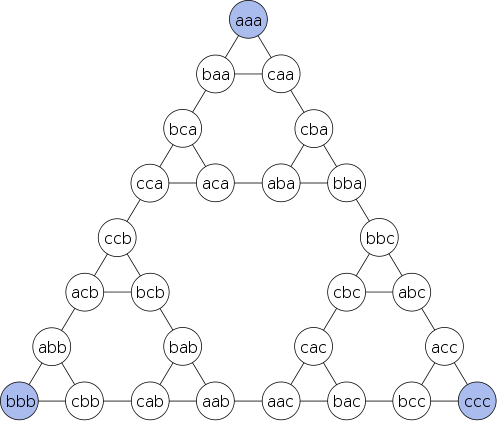
\includegraphics[width=0.9\textwidth]{img/hanoi_graph}
    \vfill
  \end{columns}
\end{frame}

\section{Data Structures}
\subsection{Basics}
\begin{frame}
  \frametitle{What are data structures?}

  A data Structure (DS) is a mean of \structure{storing} and
  \structure{organizing} data. 

  \vfill

  Different Data structures have different strengths. You need to have
  a general idea of those, in order to \structure{select} and
  \structure{use} the right DS for the right problem.
\end{frame}

\begin{frame}
  \frametitle{What do you need to know about DS?}
  % What do you need to know about Data Structures?
  % Space and time complexity (insertion/removal)
  % Special Attributes
  % VERY IMPORTANT: how to implement them (sometimes just calling the correct library)
  \begin{block}{Characteristics of DS}
    \begin{itemize}
    \item Time Complexity: Insertion, Removal, Initialization, Access;
    \item Space Complexity: Repetitions of data, Empty Space;
    \item Others: Restrictions, Special behaviors;
    \end{itemize}
  \end{block}

  \begin{exampleblock}{Usage of DS}
    \begin{itemize}
    \item Is the DS in the STL or Java API? How to call it?
    \item If not, how to implement the DS?
    \item How to perform basic operations on the DS? (Modification/Sort/Search)
    \end{itemize}
  \end{exampleblock}
  
  {\small As you learn new things, don't forget to expand your library}
\end{frame}


\begin{frame}
  \frametitle{CAVEAT: When theory is important}
  % Caveat: Usage vs Theory
  % TODO: Improve this frame
  When solving programming challenges, we will normally focus more on
  the practical aspects of Data Structures (how fast it is? how to use
  it?). It is not important to us to understant WHY they work as they do.

  \bigskip

  However, for a well rounded scientist, it is important to know both
  the practical and theoretical aspects of many techniques.
\end{frame}

\subsection{Data Structure Operations}
\begin{frame}
  \frametitle{Linear Data Structures} 
  %% Important for programming contests.
  % Linear Data structure
  %% Static Array, Dynamic Array

  {\small
  One of the most common DS used in Programming Contests are. 

  \begin{block}{Linear Data Structures}
    The elements can be ordered in a linear sequence:\\
    left to right, top to down (Including multiple dimensions).
  \end{block}

  \begin{itemize}
  \item \structure{Static Array:} 
    \begin{itemize} 
    \item The size is fixed, or estimated in advance. 
    \item Native data types. Make them bigger than necessary!
    \end{itemize}
    
  \item \structure{Dynamic Array:}
    \begin{itemize}
    \item C++ STL vector / Java ArrayList;
    \item Number of elements is truly unknown;
    \item Learn how to use .iterators!
    \end{itemize}
  \end{itemize}
  }
\end{frame}

\begin{frame}
  \frametitle{Specialized Linear DSs}
  %% TODO: Add some problem examples for this slide.
  \begin{itemize}
  \item \structure{Array of Booleans (C++ bitset)}:\\
    Useful operations such as reset, set (initialization) and test (bounded access)
  \item \structure{Stack (C++ stack/Java stack)}:\\
    O(1) push and pop. Used for recursion/Postfix/Bracket matching
  \item \structure{Queue (C++ queue)}:\\
    push (to back), pop (from front), used for Breadth First Search, Topological Sorting
  \item \structure{Deque (C++ deque)}:\\
    push and pop from both ends. Used for ``sliding window'' algorithms.
  \end{itemize}
\end{frame}

% TODO: 2D arrays: usually an array of array (unless it is a
% matrix/table problems, which will be seen later)

%%%%%%%%%%%%%%%%%%%%%%%%%%%%%%%%%%

\subsection{Operations in Data Structures}

\begin{frame}
  \frametitle{Main operations in Arrays}

  When discussing linear DS, it is important to discuss two common
  actions done on them:

  \bigskip

  \begin{itemize}
    \item \structure{Sorting} -- Changing the position of items in the
      array according to some ordering.

      \bigskip

    \item \structure{Searching} -- Finding an item in an array with a
      certain value.
  \end{itemize}
\end{frame}

\begin{frame}
  \frametitle{Actions on Linear DS -- Sorting}
  %% Give unsorted stuff, sort them
  %% For programming challenges, Sorting is usually a pre-liminary step for another problem
  \begin{block}{Super formal Definition}
    \hfill Given unsorted stuff, sort them!
  \end{block}

  \bigskip

  In programming contests, sorting is usually a preliminary step:
  \begin{itemize}
  \item sort a list to facilitate searching;
  \item sort a list to find highest values;
  \item sort a list for a greedy algorithm;
  \item sort a list to calculate cumulative values;
  \item etc...
  \end{itemize}
\end{frame}

\begin{frame}[fragile,singleslide]
  \frametitle{Sorting Example -- Vito's Family (UVA 10041)}
  
  \begin{exampleblock}{Problem description}
    A gangster wants to move to a new house. The new house should have
    minimal distance from all his family, who live on the same street.
  \end{exampleblock}

  \medskip

  This program can be summarized as ``find the median of the addresses
  and calculate the distance to all the houses.''

  \medskip

  \begin{block}{}
    {\small
\begin{verbatim}
for (i = 0; i < m; i++)
{
  cin >> add[i];
} 
sort(add,add+m);
med = add[(m/2)];
\end{verbatim}}
  \end{block}
\end{frame}


% TODO: Add this frame
%\begin{frame}
%  \frametitle{Other uses for sorting}
%  
%
%% Or maybe we want to ``beautify'' some output (eg. Return the first lexographical solution)
%\end{frame}


\begin{frame}
  \frametitle{Sorting algorithms}

  You probably have heard of a large number of sorting algorithms:

  \bigskip

  \begin{itemize}
    \item \structure{$O(n^2)$ algorithms:} Bubble, Selection, Insertion sort;
    \item \structure{$O(n\text{log}n)$ algorithms:} Merge/Heap/Quicksort;
    \item \structure{$O(n)$ algorithms}: Bucket/Radix sort;
  \end{itemize}

  \smallskip

  Can you remember the main characteristics of these algorithms?

%% Many algorithms, O(n^2), O(nlogn), Special purpose algorithms, In place, not in place

%% Huge list of sorting algorithms

%% For ICPC, you usually just need: O(nlogn) algorithm which is implemented on the library
%% Collections.sort, algorithm::sort
\end{frame}

\begin{frame}
  \frametitle{How many sorting Algorithms are there?}
  \begin{columns}[c]
    \column{0.5\textwidth}
    {\tiny
    \begin{itemize}
    \item bubblesort
    \item insertion sort
    \item selection sort
    \item heapsort
    \item mergesort
    \item quicksort
    \item radix sort
    \item bin sort
    \item gnome sort
    \item library sort
    \item comb sort
    \item tree transversal
    \item sorting networks
    \item cocktail shaking sort
    \item bucket sort
    \item bogo sort
    \item bitonick sort
    \item ...
    \item And many more!
    \end{itemize}}
    \column{0.5\textwidth}
    \includegraphics<2>[width=1\textwidth]{../img/fliptable}
  \end{columns}
\end{frame}

\begin{frame}
  \frametitle{Implementing Sorting} 

  {\small 
    You don't need to know every one of those methods. At least for
    programming contest, you need a good idea of how to use sorting in
    your language's API

    \medskip
    
  %% For ICPC, you usually just need: O(nlogn) algorithm which is implemented on the library
  %% Collections.sort, algorithm::sort
  \begin{block}{C++}
    Sorting is implemented by \emph{STL algorithm}.\\
    Eg: sort(memory\_start,memory\_end,function)\\
    See also partial\_sort() and stable\_sort()
  \end{block}
  \begin{block}{Java}
    To sort with Java we use ``Collections.sort(array,function)''    
  \end{block}
  }
\end{frame}

\begin{frame}
  \frametitle{Relax time}
  \begin{enumerate}
  \item The song of the sorting people;
    \vfill
  \item The quantum bogosort;
  \end{enumerate}
\end{frame}


\begin{frame}
  \frametitle{Searching in an array}

  \begin{block}{Finding the highest value}
    \begin{itemize}
    \item Unsorted array: $O(n)$
    \item Sorted array: $O(nlogn + 1)$
    \end{itemize}
    What if we need to repeat the operation $k$ times?
  \end{block}

  \begin{block}{Finding a specific value}
    \begin{itemize}
    \item Unsorted array: $O(n)$
    \item Sorted array: $O(n\text{log}n + \text{log}n)$ -- binary search!
    \end{itemize}
  \end{block}

  But can you implement a sorted array quickly?
\end{frame}



\begin{frame}[fragile,singleframe]
  \frametitle{Binary Search in C++}
  
  {\small You can use algorithm::lower\_bound and algorithm::upper\_bound
  
 
  \begin{block}{}
\begin{verbatim} 
#include <iostream>     
#include <algorithm>    
#include <vector>       
int main () {
  int myints[] = {10,20,30,30,20,10,10,20};
  std::vector<int> v(myints,myints+8);           
  std::sort (v.begin(), v.end());                

  std::vector<int>::iterator low,up;
  low=std::lower_bound (v.begin(), v.end(), 20); 
  up= std::upper_bound (v.begin(), v.end(), 20); 

  std::cout << "lower at " << (low- v.begin()) << '\n';
  std::cout << "upper at " << (up - v.begin()) << '\n';

  return 0; // up and low are memory indexes.
}
\end{verbatim}
    \end{block}
}

\end{frame}

%%%%%%%%%%%%%%%%%%%%%%%%%%%%%%%%%%%%%%%%%%%%

\subsection{Non Linear Data Structures}
\begin{frame}
  \frametitle{Non Linear Data Structures}

  \begin{block}{Balanced Binary Search Tree}
    \begin{itemize}
    \item C++ Map/Set (implemented as RB tree)
    \item Java TreeMap/TreeSet
    \end{itemize}
    Access/Deletion/Search in $O(\text{log}n)$.
  \end{block}

  \begin{block}{Heap}
    \begin{itemize}
      \item C++ priority\_queue
      \item Java PriorityQueue
    \end{itemize}
    Gets the highest value individual in $O(1)$
  \end{block}
\end{frame}

\begin{frame}
  \frametitle{Tree Linear Structures: Example Problem}
  \begin{block}{UVA 10226 -- Hardwood Species}
    Input is up to 1.000.000 trees, up to 10.000 types. Sort and
    output the speciation. Test cases are not limited.
  \end{block}
  
  \bigskip

  Because of the huge numbers, storing the trees in an array will not
  be enough.  We need a fast data structure to solve this problem in
  time.

  Otherwise the problem is not actually difficult.
  %% TODO: Add an illustration to the problem.
\end{frame}

%%% TODO: Extra explanation of other data sets (include problems too!)

%% Hash table
%% O(1) for insert, search, delete (if hash map is good!)
%% No hashmap on STL, but java API has one. 
%% Usually MAP (O log n) is good enough

%%%% Extras: Direct addressing table, Heap
%%%% Future classes: Graphs, Trees (Fenwick tree, segment tree), Tables

%% TODO: Graph description on Chapter 2 to be added to the Graph chapter
%% Union-find also to add to graph chapter

%%%%%%%%%%%%%%%%%%%% BITSET %%%%%%%%%%%%%%%%%%%%%%%%%%%%%%%%%%%%%%

\section{End Friday}
\subsection{Conclusion Friday}
\begin{frame}
  \frametitle{Conclusion and problems}
  
  \begin{itemize}
  \item Seven problems are listed, all of them related to DS;
  \item However, you don't need to solve ALL of them (unless you want
    to!)
  \item Try to discover which problems are easier, and solve those
    first.
  \end{itemize}

\end{frame}

\subsection{Bonus}
% Sort algorithm songs
% Bill gates flapjacks % Sorting too (maybe search?)./\

%\section{Bitset}
%
%\begin{frame}
%\end{frame}

%\subsection{Conclusion Monday}

%% Take from book
%\begin{frame}
%\end{frame}


\section{Old Slides}
\subsection{Old Slides}

\begin{frame}
  \frametitle{Know your data structures!}
  \begin{block}{}
    To be able to do data structure tricks, we need to be familiar
    with a variety of data structures.
  \end{block}

  \bigskip

  \begin{itemize}
  \item What is the time and memory efficiency of each data structure?
  \item What is \structure{programming efficiency} of each data structure?
  \item What are the common uses?
  \item What are the common bugs?
  \end{itemize}
  
\end{frame}

\begin{frame}
  \frametitle{Data Structure Libraries}

  The ``Library'' word can have many meanings:

  \begin{block}{Language Library}
    \begin{itemize}
    \item What function is used to create a dictionary?
    \item What parameters are passed in this function?
    \end{itemize}
  \end{block}

  \begin{block}{Personal Library}
    \begin{itemize}
    \item How many data structures do you personally remember?
    \item Notes on paper can be very useful!
    \end{itemize}
  \end{block}
\end{frame}

\begin{frame}
  \frametitle{Low Level Data Structures}
  \begin{itemize}
  \item Array
    \vspace{.5cm}
  \item Linked List
  \end{itemize}
  
  \bigskip

  \begin{block}{}
    The Array is usually simpler, and less bug prone. But be careful with
    index overflows!
    \medskip
    
    When in doubt, use a bigger array!
  \end{block}
\end{frame}

\begin{frame}
  \frametitle{Medium Level Data Structures}
  \begin{itemize}
  \item Stack
    \vspace{.5cm}
  \item Queue
  \end{itemize}

  \bigskip

  \begin{block}{}
    The stack is the simplest ``complex'' data structure. It is
    implemented with an array and an index.
    \medskip
    
    How do you implement a Queue using two stacks?
    \medskip

    Queue and Stack are used very often.
  \end{block}
\end{frame}

\begin{frame}
  \frametitle{High level data structures}
  \begin{itemize}
  \item Sets
  \item Dictionaries
  \item Priority Queues
  \end{itemize}
  
  \bigskip

  \begin{block}{}
    These structures attach extra information to data: Key,
    Uniqueness, order.
    \medskip

    Try to think of them as combinations of the above techniques. How
    would you implement them?
  \end{block}
\end{frame}

\begin{frame}
  \frametitle{Other data structures}
  \begin{itemize}
  \item Trees
  \item Graphs
  \end{itemize}

  \bigskip

  We well talk about these in future classes
\end{frame}

\subsection{Strings}

\begin{frame}
  \frametitle{String Representation in Computers} 
  When you tyle ``\emph{ls}'', why do numbers appear before letters?

  \bigskip
  
  \begin{block}{}
    Strings in a computer system are represented as an
    \structure{Array of characters}, and each character is represented
    as an index.
  \end{block}
\end{frame}

\begin{frame}
  \frametitle{Characters as numerical indexes: what are the consequences?}
  \begin{itemize}
  \item Operation on characters (Addition, comparison);
  \item Arbitrary order of glyphs;
  \end{itemize}
\end{frame}

\begin{frame}
  \frametitle{Encodings}
  \begin{block}{}
    Encodings are mappings between a set of indexes and a set of
    glyphs. Different encodings cause Mojibake.
  \end{block}

  \medskip

  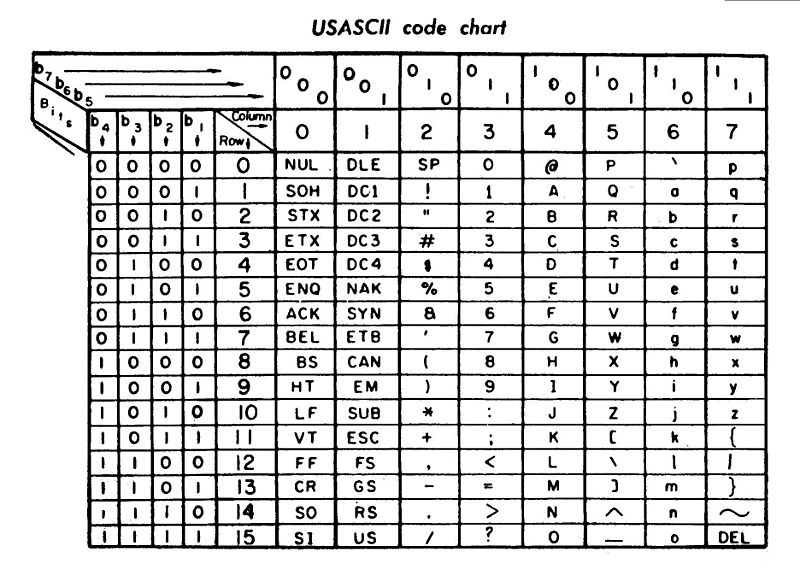
\includegraphics[width=0.7\textwidth]{img/ASCIItableOld}

  \medskip

  ASCII Indexes were selected with very specific properties.
  
\end{frame}

%%%%%%%%%%%%%%%%%%
% TODO: 
\end{document}
